\documentclass[a4paper,14pt]{extreport}
\usepackage[T1]{fontenc}
\usepackage[table]{xcolor}
\usepackage{titlesec}
\usepackage{graphicx}
\usepackage{float}
\usepackage{amsmath}
\usepackage{hyperref}
%\usepackage{amsthm}
\usepackage{mathtools}
%\usepackage{fancyvrb}
\usepackage[colorinlistoftodos]{todonotes}
\usepackage[english]{babel}
%\usepackage{csquotes}
\usepackage{hyperref}
\usepackage{neuralnetwork}
\usepackage{quoting}
\usepackage{changepage}

\begin{document}

% First page
\title{
	{{\large{\textsc{Alma Mater Studiorum $\cdot$ University of Bologna}}}}
	\rule{\textwidth}{0.4pt}\vspace{3mm}
	\textbf{Flatland Challenge}
	
	Deep learning course final project
}

\author{Lorenzo borelli (\href{mailto:lorenzo.borelli@studio.unibo.it}{lorenzo.borelli@studio.unibo.it}) 
\\ Giovanni Minelli (\href{mailto:giovanni.minelli2@studio.unibo.it}{giovanni.minelli2@studio.unibo.it}) 
\\ Lorenzo Turrini(\href{mailto:lorenzo.turrini4@studio.unibo.it}{lorenzo.turrini4@studio.unibo.it})}
\date{\today}
\maketitle
\newpage
\tableofcontents
\listoffigures
\listoftables
\newpage

\chapter{Introduction}
The \textbf{Flatland challenge} consists in tackling the vehicle scheduling problem, in a controlled and simulated environment. The main approach used here is reinforcement learning, however there are several other possibilities that fall under the umbrella of combinatorial optimization.\\
The aim of the challenge, from a RL standpoint, is to allow the agents to learn how to optimally reach their target in minimal time.

\chapter{The environment}
\section{Railway network}
The flatland environment is simulated by a rectangular grid of fixed size, which can be set by the user. Each cell of the grid is either a rail cell, or an empty unusable cell, or a \textbf{target} cell. Rails are of different type, depending on the available \textbf{transitions}: there are 16 different transitions in flatland, since there are 4 different orientations, and 4 other directions of exit from the cell. Thus, each cell is described by a bitmap that represents the whole transition space.\\
However, not every transition is allowed in flatland.\ Since the aim is to actually simulate a real railway system, only a maximum of 2 exit directions are allowed from every orientation of the agent, which result in 8 different cell types (including empty ones).\\ \\
Flatland offers also a \textit{sparse\_rail\_generator} that randomizes the creation of a realistic railway structure, where clusters of cities are sparsely connected to each other, allowing to mimic as faithfully as possible real city railway networks.

\begin{figure}[H] 
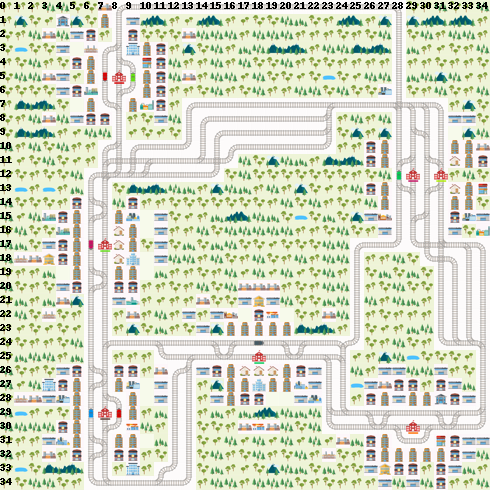
\includegraphics[height=80mm, width=80mm, scale=0.5]{figures/sparse_railway.png}
\centering
\caption{Sparse railway}
\label{fig:s1}
\end{figure}

\section{Agents}
Trains have a number of important properties:
\begin{itemize}
\item \textbf{Position}: the current coordinates of the agent.
\item \textbf{Target}: the position of the target cell.
\item \textbf{Direction}: the current orientation described with an integer\\
    \verb|[0=North, 1=Est, 2=South, 3=West]|
\item \textbf{Movement}: an integer describing the status of the agent\\
    \verb|[0=READY_TO_DEPART, 1=ACTIVE, 2=DONE, 3=DONE_REMOVED]|
\end{itemize}
\noindent
Since every agent is liable to malfunctions, much like real trains, there are properties to keep track of that in addition to variables that store the agents' speed:
\begin{itemize}
\item \textbf{Malfunction rate}: the Poisson rate at which malfunctions occur
\item \textbf{Malfunction}: a counter of the remaining time the agent will remain malfunctioning
\item \textbf{Next malfunction}: number of steps until next malfunction will occour
\item \textbf{Number of malfunctions}: the total number of malfunctions for this agent
\item \textbf{Max speed}: a fraction between 0 and 1. (\textit{e.g.} a speed of 1/2 means that the agent changes cell after 2 time steps)
\item \textbf{Position fraction}: related to speed, indicates when the next action can be taken
\end{itemize}
\section{Environment Actions}
\label{sec:envActions}
The available actions are:
\begin{itemize}
\item \textbf{DO NOTHING (0)}: Default action if None has been provided or the value is not within this list. If agent.moving is True then the agent will \textit{MOVE\_FORWARD}.

\item \textbf{MOVE LEFT (1)}: If the transitions of the current cell allows it, the agent change its direction towards the left, otherwise the action is masked with a \textit{MOVE\_FORWARD}. If the agent is not moving then update also it's state to moving.

\item \textbf{MOVE FORWARD (2)}: It updates the direction of the agent following the transitions allowed in the current cell. If the cell is a dead-end the new direction is the opposite of the current. If the agent is not moving then update also it's state to moving.

\item \textbf{MOVE RIGHT (3)}: If the transitions of the current cell allows it, the agent change it's direction toward the right, otherwise the action is masked with a \textit{MOVE\_FORWARD}. If the agent is not moving then update also its state to moving.

\item \textbf{STOP MOVING (4)}: Stop the agent in the current occupied cell and cause the change of value of the variable describing the state of the agent.

\end{itemize}
\section{Rewards}
\label{sec:envRewards}
The rewards are based on the following values:
\begin{itemize}
\item \textit{invalid action}: penalty which is currently set to 0, penalty for requesting an invalid action
\item \textit{step penalty}: which is -1 * alpha, penalty for a time step.
\item \textit{global reward}: calculated as 1 * beta, a sort of default reward.
\item \textit{stop penalty}: is currently set to 0, penalty for stopping a moving agent
\item \textit{start penalty}: is currently set to 0, penalty for starting a stopped agent
\end{itemize}
The full step penalty is computed as the product between \textit{step penalty} and agent speed data (\textit{i.e.} the \textit{speed} variable).\
There are different rewards for different situations:
\begin{itemize}
\item agents that are in status \textit{DONE} or \textit{DONE\_REMOVED} have zero reward.
\item all agents that have finished in this episode (checked at the end of the step), have reward equal to the global reward (when in step all agents have reached their target)

\item full step penalty is assigned when an agent is in state \textit{READY\_TO\_DEPART} and in the current turn moves or stay there (2th step agent case), or when is in malfunction.
\item full step penalty plus the other penalties (invalid action penalty, stop penalty and start penalty) when the agent is finishing actions or start new ones. Currently the other penalties are all set to zero.
\end{itemize}
The end of the Each train starts counting rewards since the beginning, not since it becomes \textit{ACTIVE}. Currently it is possible to say that agents’ rewards are always full step, excluding when the episode ends and when they have finished, where is 0.



\chapter{Our environment}
Our flatland environment is based on the base RailEnv class and there we wrapped the main functionalities and ease the interaction from the other classes. In order to parametrize as possible the env details we also used a file yaml \textit{"env$\_$parameters.yml"}.\\
The main functionalities are:
\todo{manca il metodo dentro gli utils per la creazione dell'env e la descrizione dei controller}
%we have implemented some environmental controller to flexibly add and/or remove various features in the train/evaluation phase, preserving the original Flatland’s implementation. Since the controllers are tied to the solving approach they passed from the main as parameters and instantiated inside the Flatland RailEnv class. However our implementation of the two proposed approaches share the same controller since the same features are observed and the main configuration can be tuned just acting on the parameters inside the .yml files.

\begin{itemize}
\item \textbf{step}: in this method, there were calculated observations, standard rewards, standard info and the list of agents which have finished their run, through super method of the environment.
Then, our custom actions are performed on the dictonaries before the return of the step results.\ Additional information are extracted from he observations and encoded in the information dictionary with method \textit{extract\_info} since they will be necessary for the following steps. The deadlock situation is updated with the aid of the deadlock controller, and rewards and statistics are computed properly. At the end a normalization procedure for the observations is applied in order to feed the training model.
\item \textbf{extract info}: it takes as parameters the information and observation, which are used to fill the following variables included in the dictionary as additional information:
\begin{itemize}
\item \textit{decision\_required}: this variable is used to determine if agent is into a switch so the observation is not None. This flag for every agent, if is true it allows to call the act of the policy.
\item \textit{shortest\_path}: this variable is a list of minimum number of switch remain to arrive at target for every agent. It is used to calculate rewards to determine if the agent come near in at target as compared to previous step.
\item \textit{shortest\_path\_cost}: this variable is a list of minimum distance remain to arrive at target for every agent.
\item \textit{shortest\_path\_pre}: this variable is a list of minimum numebr of switch remain to arrive at target for every agent in previous step. It is used to calculate rewards to determine if the agent come near in at target as compared to current step.
\item \textit{shortest\_path\_pre\_cost}: this variable is a list of minimum distance remain to arrive at target for every agent in previous step.
\end{itemize}
\item \textbf{reset}: in this method, the info and observation are reset at start state through super method of the environment of flatland. Consequentially they are reset also the external controllers for deadlock and statistics management. This method is called at the end of every episode.
\item \textbf{render env}: in this method through a parameter, it is launched the graphic interface.
\end{itemize}
\section{Parameters}
There is a file \texttt{env\_parameters.yml} that contains all configurations of our environments. In details it contains three type of environments defined by us for testing purpose:
\begin{enumerate}
	\item [1.] Small size:
	\begin{itemize}
		\item $n\_agents: 3$
		\item $width: 40$
		\item $height: 40$
		\item $n\_cities: 2$
		\item $max\_rails\_between\_cities: 2$
		\item $max\_rails\_in\_city: 3$
		\item  $variable\_speed: False$
		\item $malfunctions\_enabled: True$
		\item $malfunction\_rate: 0.005$
		\item $min\_duration: 20$
		\item $max\_duration: 50$
		\item $max\_state\_size: 24$
	\end{itemize}
	\item [2.] Medium size:
		\begin{itemize}
		\item $n\_agents: 7 $
		\item $width: 60 $
		\item $height: 60 $
		\item $n\_cities: 5 $
		\item $max\_rails\_between\_cities: 2 $
		\item $max\_rails\_in\_city: 3 $
		\item  $variable\_speed: False $
		\item $malfunctions\_enabled: True $
		\item $malfunction\_rate: 0.005 $
		\item $min\_duration: 15 $
		\item $max\_duration: 50 $
		\item $max\_state\_size: 48$
	\end{itemize}
	\item [3.] Big size:
		\begin{itemize}
		\item $n\_agents: 10 $
		\item $width: 80 $
		\item $height: 80 $
		\item $n\_cities: 9 $
		\item $max\_rails\_between\_cities: 5 $
		\item $max\_rails\_in\_city: 5 $
		\item  $variable\_speed: False $
		\item $malfunctions\_enabled: True $
		\item $malfunction\_rate: 0.0125 $
		\item $min\_duration: 20 $
		\item $max\_duration: 50 $
		\item $max\_state\_size: 72$
	\end{itemize}
\end{enumerate}
In addition there are a some parameters to calculate the rewards:
\begin{enumerate}
	\item Rewards:
	\begin{itemize}
		\item $deadlock\_penalty: -10$
		\item $starvation\_penalty: -0.5$
		\item $goal\_reward: 10$
		\item $reduce\_distance\_penalty: 0.5$
	\end{itemize}
\end{enumerate}
\section{Metrics}
The metrics are fundamental to understand how enviroment and policy are behaving so  We implemented a \texttt{StatisticsController} to compute and print the metrics and evaluate the algorithm’s performance:
\begin{itemize}
	\item \textbf{normalized\_score}: is the sum of the rewards accumulated by all agents during the episode divided by the worst score obtainable, computed as the product between the number of agents and the maximum number of steps in the episode.
	In the worst case, all agents do not reach their destination, therefore for each step they get a negative reward.
	\begin{equation}{\frac{score}{max\_steps \cdot n\_agents}}\label{eq:score}\end{equation}
	\item \textbf{accumulated\_normalized\_score}: is the mean of \textbf{normalized\_score} obtained up to that point.
	\begin{equation}{\frac{\sum{normalized\_score}}{N}}\label{eq:score_acc}\end{equation}
	\item \textbf{completion\_percentage}: is the percentage of agents who reached their destination in the episode.
	\begin{equation}{100 \cdot {\frac{tasks\_finished}{n\_agents}}}\label{eq:compl_perc}\end{equation}
	\item \textbf{accumulated\_completion}: is the mean of \textbf{completion\_percentage} obtained up to that point.
	\begin{equation}{\frac{\sum{completion\_percentage}}{N}}\label{eq:compl_acc}\end{equation}
	\item \textbf{deadlocks\_percentage}: is the percentage of deadlocks that occurred in the episode.
	\begin{equation}{100 \cdot {\frac{n\_deadlocks}{n\_agents}}}\label{eq:deads_perc}\end{equation}
	\item \textbf{accumulated\_deadlocks}: is the mean of \textbf{deadlocks\_percentage} obtained up to that point.
	\begin{equation}{\frac{\sum {deadlocks\_percentage}}{N}}\label{eq:deads_acc}\end{equation}
\end{itemize}
The \texttt{StatisticsController} also computes the probability distribution of the actions taken during each episode.
We integrated our solution with \textbf{TensorBoard} in order to be able to analyze the evolution of both training data (losses, expected values, memory sizes, exploration rates \ldots) and performance metrics.
\section{Evaluation and platforms}
To run the experiments we did have at our disposal our personal computers which are enought powerful to not represent a limitation for smaller environments therefore  we didn't faced a lot of difficulties for the initial debug of the code and the firsts tests for the decision of the metrics. In bigger instances primary focused to the evaluation of the models we instead experienced a slowdown in the running times. We observed that the major bottlenecks are in the Flatland code for which it is necessary to have more CPU power.\\
Due to this reasons we decided to limit the complexity of the experiments especially in terms of number of agent and map size, considering just the following environments with test sessions of 1000 iterations each.
\begin{enumerate}
	\item Medium size: 60x60
	\item Big size: 80x80
\end{enumerate}
\todo{fai bene l'internal link alla sezione...}
\textit{(detailed features of each one can be found in \hyperref[sec:ourParameters])}.\\
In order to evaluate different algorithms, combinations of hyperparameters and strategies we looked for a tool able to store, track, share and effectively compare different runs without the worry of continuously make notes on external files of our progresses.
We found such a tool in \href{https://www.wandb.com/}{Weights \& Biases}.
Subscribing to a free account provides an effective and very intuitive way of monitoring a Deep Learning project.\\
Weights \& Biases is used by OpenAI and other leading companies since it's wide range of supported platforms. Indeed we were able to integrate it rapidly in the project, connecting it to the TensorBoard logging and immediately start testing.\\
Additionally to a rich customizable interface to plot graphs it also provides hyperparameter tuning, called Sweep.
\todo{we have to add more about the seep?}
\todo{review initial here}
\section{Action}
The Flatland environment provides for each agent five different actions (already described in detail in \hyperref[sec:envActions]{2.3}).\\
In the implementation phase we reasoned about the utility of each one in order to possibly reduce the action space that our RL model has to learn.
The \texttt{DO\_NOTHING} is not necessary to reach a solution, because the behaviour of an agent can easily manipulated changing his movement status from the action \texttt{STOP\_MOVING} or \texttt{MOVE\_FORWARD}. Hence being useless and possibly damaging the overall performance we decided to consider its removal. Thinking further, the \texttt{MOVE\_LEFT} and \texttt{MOVE\_RIGHT} actions can be thought as ambiguous command actions where they are forbidden, since the environment will automatically mask them as forward commands. Therefore it is natural to conclude that the agents may learn bad policies that maps these actions to the same effect of the \texttt{MOVE\_FORWARD} action. That, has been observed as a very common phenomenon due to the presence of long straight paths where the agent is allowed only to stop or move forward. Anyway even the stop action in the middle of the rail does not have much sense since the unique good reason to perform a stop voluntary would be the one of give the precedence, and that can happen only in proximity of a switch cell. \\
For this reason we considered the possibility to force agents to only decide and learn before and over switches, where multiple actions are allowed and agents may learn to give way to other agents, avoid deadlocks, reach the target and more. This considerations lead to skip a lot of choices during learning and deploy a strategy of action masking to avoid illegal actions.
An alternative, very common, strategy to address invalid actions would be the one of applying negative rewards, but this also requires the agent to explore the actions and understand how to map actions to the possibility of applying them resulting in a much more longer training time and the possibility that the agent converges to a wrong policy. Invalid action masking, instead, helps to avoid sampling invalid actions by “masking out” the network outcomes corresponding to the invalid actions. \\
Following our reasoning we evaluate the action only before or on the switch and in these case there is a flag \textit{decision\_required} equals True.
\begin{itemize}
\item \textbf{"decision\_required" = True}: the action choice is up to the policy on the basis of the observation provided.
\item \textbf{"decision\_required" = False}: the action is decided by the environment. Assigning the constant \texttt{RailEnvActions.MOVE\_FORWARD} the agent will continue on the road following the direction of the road.
\end{itemize}
\section{Deadlock Controller}
In Flatland, deadlocks are a truly catastrophic event because the agents involved can no longer move and can represent an obstacle for the others during the rest of the episode. Deadlocks detection is an additional riddle in the Flatland for which there is no standard algorithm. We have tried to implement a detection system as efficient as possible able to identify failures and conflict states with the minimum overhead. That was possible especially with the aid of a custom observation. Overall, we have implented two type of detection systems based on the type of observation used.
\begin{itemize}
	\item \textbf{DeadlocksGraphController}: this controller is used in combination of a graph structured observation. It make use of the observations of each agent controlling the presence of labels in the in the graph nodes, for instance the observation of an agent in a deadlock situation will contain a node marked with the \texttt{DEADLOCK} label.\\ Remarking that for this type of observation each node represent a switch in the rail, we decided to mark a node as deadlock when an agent taking a road, with his direction of movement, will surely face another agent in opposite direction. This type of observation however is irremediable and can develop only in a full deadlock status when both agents in the road are one next to the other. That data can be found in the same labeled node under the name of \textit{steps\_to\_deadlock}. When that value is 0, coherently, the list maintained to register the deadlock status of the agents is updated, and these agents won't be considered anymore in the next steps.\\
	To prevent such situation the model is required to learn with the aid of conflict nodes in the observation. Such label (\texttt{CONFLICT}) means that there is a possibility to have a deadlock situation for the current agent taking the direction of that switch because there is at least another agent facing that switch.\\
	The \texttt{STARVATION} label assignment suggest instead a situation in which an agent is not able to arrive to his target position. That is possible for example in cases where two agents or more are in deadlock and block the unique road available to reach a station. When such label is present in the observation the agent situation can only develop to a deadlock status but the RL model shouldn't be penalized for that because no other option would be available. In such case we decided also to change the target to the nearest deadlock position with the objective to not cause more damages to other agents.
	This implementation of the deadlock controller allow also to interrupt an episode early when all the agents are in \texttt{DONE} status or \texttt{DEADLOCK} or \texttt{STARVATION}.
	\item \textbf{DeadlocksController}: this controller is the default used with any type of observation. It use the distance matrix for determinate if an agent is in deadlock, checking adjacent cell and comparing directions of other agent. In case of a deadlock, the corresponding flag of the agents involved is marked true. In this implementation hasn't been taken care of the conflicts or starvation situations, since they will in any case develop in a deadlock or being interrupted by the end of episode. This obviously involves an higher risk to incur in deadlock cases or slow down other agents and in a deterioration of network performance but is more simple.
\end{itemize}
\section{Rewards}
As mentioned before \hyperref[sec:envRewards]{2.4} the Flatland environment provides a basic rewards system briefly describable with the following points:
\begin{itemize}
	\item Every step agent receives a negative reward proportionate to his speed if he has not reached his destination.
	\item Each agent receives a reward equal to 0 if he has reached his destination.
	\item If all agents have reached their destination they receive a reward equal to 1.
\end{itemize}
We think that this reward system is lacking of some important details to fully represent the complexity of the problem because there is not much distinction between the states in which the agents may be while navigating in the environment.\\
Intuitively an agent have to learn two behaviors, not necessarily in this order:
\begin{itemize}
	\item Reach his destination in the shortest time possible.
	\item Avoid collisions with other agents.
\end{itemize}
Let's consider a small environment with 3 agents, in this case the main behavior is the first because the probability of a collision is not very relevant, but if we consider the same environment with 10 agents the skill to avoid deadlocks is decisive for the overall performance.\\
According to the Flatland's rewards system there is not difference between being deadlocked and navigating the map without reaching destination from an agent's point of view in terms of rewards. \\
In order to stimulate the learning of the desired behaviors we have tried to modify the Flatland's rewards system by using a method known in literature with the name of \textbf{Reward Shaping}.
Crafting rewards is not easy because as a consequence we could get trapped in the "Cobra Effect":

\begin{quoting}[font=itshape, begintext={"}, endtext={ \footnote{https://medium.com/@BonsaiAI/deep-reinforcement-learning-models-tips-tricks-for-writing-reward-functions-a84fe525e8e0}}]
	Historically, the government tried to incentivize people to assist them in ridding the area of cobras.
	If citizens brought in a venomous snake they had killed, the government would give you some money.
	Naturally, people started breeding venomous snakes.
\end{quoting}

Indeed, this method may cause an undesirable effect: stimulating the learning of one behavior can cause the learning of another wrong.\\
Taking all of that in consideration, in our implementation we added a method in the env class called \textbf{compute$\_$rewards} to flexibly choose during the training phase whether to use the rewards shaped or the standard Flatland's reward system.\\
In the first case it is possible to choose how to shape the rewards by setting the following parameters:
\todo{la tre non l'ho capita}
\begin{itemize}
	\item\textbf{$deadlock\_penalty$}: to penalize agents in deadlocks by value of variable.
	\item \textbf{$starvation\_penalty$}: to penalize agents in starvation by value of variable.
	\item \textbf{$reduce\_distance\_penalty$}: to reward agents who are moving towards their target by multiplying the value assigned to the reward associated with the agent calculated in the previous step.
	\item \textbf{$goal\_reward$}: to reward agents who have arrived at their destination by assigning them a positive reward.
\end{itemize}


\chapter{Reinforcement learning}
\textbf{Reinforcement learning} aims at training agents that operate in an environment by assigning rewards to their actions. Agents decide which action to take based on a \textbf{policy} $\pi(a_t, s_t)$, with $s_t$ being the observation of the environment at time step t. \\
Maximizing the sum of rewards is the method whereby the agent improves the policy and learns.

\section{DQN}
\cite{dqn} described a network model to approximate the Q-function $Q^{\pi}(s,a)$, which measures, for each state-action pair, the discounted sum of rewards, following from the policy $\pi$. The optimal Q-function, that is the maximum reward which can be obtained by performing a certain action a in state s, obeys the \textbf{Bellman optimality equation} $$Q^*(s,a) = E[r + \gamma max_{a'}Q^*(s', a')]$$
It follows that the maximum return is obtained by the immediate reward and the discounted return that the agent gets by following the policy; in practice, however, neural networks are needed in order to avoid computing a huge Q-table, and they are trained by minimizing the \textbf{temporal difference} loss, that is the difference between the current prediction and the expected optimal target.  
We started by implementing a slight variation of DQN as described in \cite{dqn}, without the use of CNN, but by simply using fully connected layers with \textbf{ReLU}, which take as input a vector representation of the graph as processed by the GCN, since we felt that classic convolution wouldn't be very effective in this environment. \\
\begin{center}
\begin{neuralnetwork} [nodespacing=10mm, layerspacing=25mm,
			maintitleheight=2.5em, layertitleheight=2.5em,
			height=5, toprow=false, nodesize=17pt, style={},
			title={}, titlestyle={}]
		% nodespacing = vertical spacing between nodes
		% layerspacing = horizontal spacing between layers
		% maintitleheight = space reserved for main title
		% layertitleheight = space reserved for layer titles
		% height = max nodes in any one layer [REQUIRED]
		% toprow = top row in node space reserved for bias nodes
		% nodesize = size of nodes
		% style = style for internal "tikzpicture" environment
		% titlestyle = style for main title
		        \newcommand{\x}[2]{$s_#2$}
		        \newcommand{\y}[2]{$\hat{Q}_#2$}
		        \newcommand{\hfirst}[2]{\small $h^{(1)}_#2$}
		        \newcommand{\hsecond}[2]{\small $h^{(2)}_#2$}
		        \inputlayer[count=3, bias=true, title=Input\\layer, text=\x]
		        \hiddenlayer[count=4, bias=false, title=Hidden\\layer 1, text=\hfirst] \linklayers
		        \hiddenlayer[count=3, bias=false, title=Hidden\\layer 2, text=\hsecond] \linklayers
		        \outputlayer[count=5, title=Output\\layer, text=\y] \linklayers
\end{neuralnetwork}
\end{center}
	
\noindent 
The units in the hidden layers default to 64, but the dimensions and the number of layers are fully customizable by the user, while the input layer is just made by the state of the environment, and the output layer has as many units as there are actions in flatland. \\ The \textit{Model} class implements the neural network, using \textbf{Huber loss} and \textbf{Kaiming initialization}. The former is, as explained in \cite{huber}, a loss function that clips the gradient to the $[-1,1]$ interval, avoiding \textbf{exploding gradient}. While on one hand it behaves like the absolute loss, for small errors it is more similar to the squared loss, thus combining the properties of both losses, while circumventing the problem of outliers which plagues the squared loss.\\
\begin{figure}[H] 
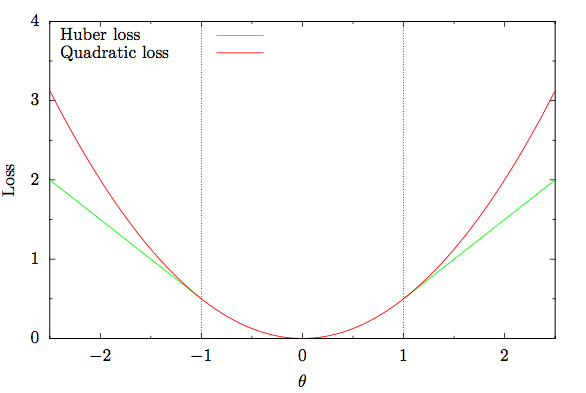
\includegraphics[height=80mm, width=100mm, scale=0.5]{figures/huber.png}
\centering
\caption{Huber and squared loss}
\label{fig:s2} 
\end{figure}
\noindent
 \\ Kaiming initialization is instead a method for weights matrix initialization, described in \cite{kaiming}, which draws samples from a standard normal distribution, to avoid \textbf{vanishing} and \textbf{exploding gradient}, and then adjusts this distribution to the ReLU activation function. It does so by doubling the variance, since ReLU halves it w.r.t. to the original standard normal distribution (see \ref{fig:s3}).
 
 \begin{figure}[H] 
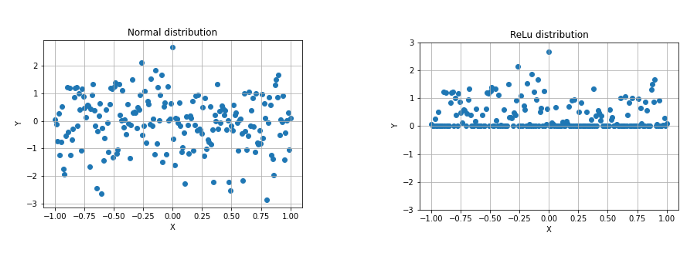
\includegraphics[height=80mm, width=140mm, scale=0.5]{figures/relu_dist.png}
\centering
\caption{Normal and ReLU distributions}
\label{fig:s3} 
\end{figure}

\noindent
\\
The \textit{DQNPolicy} class implements the main methods needed for the training loop:
\begin{itemize}
\item \textbf{act}: implements the \textbf{$\epsilon$-greedy} action selection policy, by generating a random number, and then comparing it with $\epsilon$. This hyperparameter is then iteratively decreased at the end of each episode in order to incrementally rise the probability of allowing the model itself to pick the action.
\item \textbf{step}: performs the learning step, though only once every \textit{update\_rate} time steps, a hyperparameter initialized in the yml configuration file. Before that, if prioritized experience replay is used, then the priority is computed and the current experience tuple stored in memory with that priority.
\item \textbf{learn}: called by the step method, it actually performs the learning step with an experience sampled by the memory. It computes the temporal difference target and then performs a gradient descent step. It also updates the memory with the newly computed temporal difference, which serves as a priority for the experiences.
\end{itemize}

\noindent
We also used a technique called \textbf{Fixed Q-targets}.\\
Since in a reinforcement learning setting we do not have target values prepared, we would need to use the same network for both the model's weights and for the target, leading to instability of the target values. Thus, we use 2 equal networks, one to just compute the target Q value, and the other for training. Every 100 time step, a tunable hyperparameter, the target network is \textit{soft updated} with a portion of the current weights determined by this formula $$\theta_i = \tau * \theta_i + (1 - \tau) * \theta_i$$ and by the hyperparameter $\tau$. 

\subsection{Experience replay}
Past experiences are recorded in a memory buffer that is sampled, when needed, to train the network. We implemented two different variations: \textbf{random} and \textbf{prioritized experience replay}, as explained in \cite{priority}. The paper illustrates greedy and stochastic prioritization: both leverage priority based on \textbf{temporal difference}, but the latter is more robust, allowing to replay every experience in the buffer at least once; instead, greedy prioritization risks overfitting since the same higher priority experiences are always replayed. \\
\noindent
Concretely, in stochastic prioritization, the probability to sample transition $i$ is $$P(i) = \frac{p_i^\alpha}{\sum_k p_k^\alpha}$$ with $p_i = temporal\ difference\ + \epsilon$. \\
$\alpha$ is a hyperparameter that controls the tradeoff between random ($\alpha$ = 0) and priority choice ($\alpha$ = 1), while $\epsilon$ is a small positive hyperparameter to always keep a non-zero priority, thus allowing to revisit even the lowest priority experiences: this specific variant is called \textbf{proportional stochastic prioritization}. Finally, for further stability, we added \textbf{importance-sampling weights}: for each transition $i$, weights are computed as $$w_i = (\frac{1}{N} * \frac{1}{P(i)})^\beta$$ and then fed to the Q-learning update, giving higher importance to low priority transitions, thus fixing the inherent bias of priority sampling, that favors higher priority samples. $\beta$ is used to control the amount of sampling over time, and usually reaches 1 by the end, since it's more important to have unbiased updates near convergence.\\
\noindent
This implementation uses a \textit{sum tree} data structure to store priorities and experiences, a binary tree where the leaves contain the priorities and data, while the inner nodes feature the sum of the children's priorities, with the root having the total priority: the sum tree provides $O(log(n))$ updates and sampling, with an efficient way to retrieve cumulative sums.
\noindent

 \begin{figure}[H] 
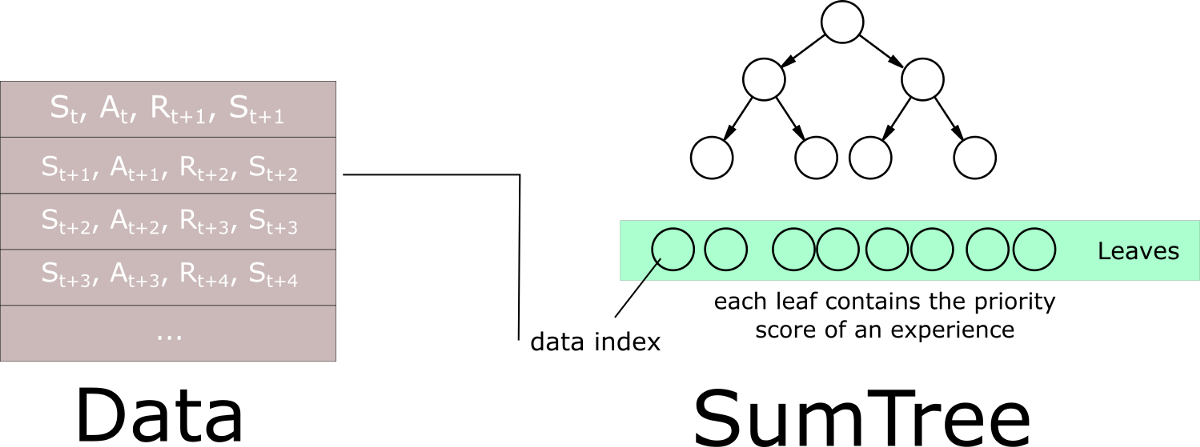
\includegraphics[height=80mm, width=140mm, scale=0.5]{figures/SumTree.png}
\centering
\caption{Sum Tree}
\label{fig:s4} 
\end{figure}
\noindent
The \textit{SumTree} class stores 2 numpy arrays, one for the experiences (so just the leaves), and the other represents the tree and thus stores the priorities. Inside the class there is a pointer to the current leaf that is constanly updated and used whenever a new experience is added to the replay memory. If the number of samples exceeds the capacity of the memory, the last experience is overwritten by the new one. \\
\textit{PrioritizedReplay} is the class implementing the probabilistic sampling of the experiences from the memory (sumtree): the total priority is divided in \textit{batch\_size} segments, so that for each element in the batch we have a segment from which we can sample uniformly a priority, which is in turn used to pick a leaf from the tree. 	

\subsection{Dueling}

The model was further improved with \textbf{dueling} architecture. The main issue of standard DQN lies in the fact that the \textbf{Bellman operator} tends to overestimate the Q value: as stated in \cite{dueling}, the solution seems to be to separate the computation of the Q value in 2 separate functions, $$Q_{\pi}(s,a) = V_{\pi}(s) + A_{\pi}(s,a) $$ The \textbf{advantage} $A(s,a)$, which computes the  ''advantage'' of taking the action a in state s w.r.t. the other possible actions in that state, and the \textbf{value} $V(s)$ which simply measures how good the state s is, regardless of the possible actions; this is particularly useful whenever we're dealing with environments that are not affected by actions in every state, like Flatland, where actions are only really relevant at switches.

\begin{figure}[H] 
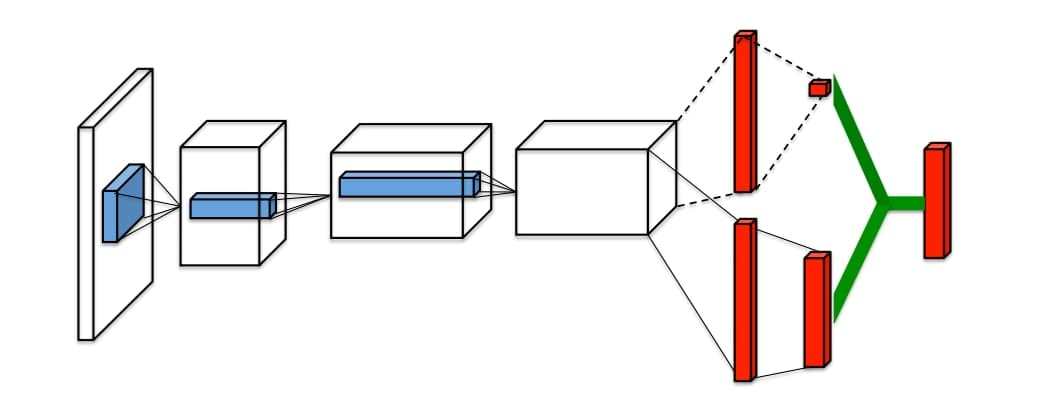
\includegraphics[height=80mm, width=140mm, scale=0.5]{figures/dueling.jpg}
\centering
\caption{Dueling DQN}
\label{fig:s5} 
\end{figure}
\noindent
Advantage and value still need to be recombined, and since the standard formula doesn't allow to extract A and V from the Q value, \cite{dueling} suggested to force the advantage to be 0 at the chosen best action, which results in the output formula for Q $$Q_{\pi}(s,a) = V_{\pi}(s) + (A_{\pi}(s,a) - max_{a' in A} A(s,a'))$$ It also highlights, however, that empirically, subtracting the average advantage yields better results.


\section{A2C}
Actor-critic algorithms, unlike \textbf{off-policy} methods that rely on local updates and transitions, like Q-learning, directly try to learn the optimal policy.\\
Assuming to parametrize the policy $\pi$, A2C introduces a \textbf{baseline}, the critic network, dependent on the state of the environment, which is essentially the value function \textbf{$V^{\pi}(s_t)$}. The policy, computed by the actor network, is evaluated w.r.t to this baseline, such that the estimator function becomes $$\nabla_{\theta} log \pi(a_t | s_t,\theta) (R_t - V^{\pi}(s_t))$$ with the difference between the reward and the baseline measuring how well the actor performed. \\ \\
In \cite{a2c}, the authors implemented an A2C algorithm to solve a DAG scheduling problem. Since we also employed a DAG as observation, we decided to implement an actor-critic network with graph normalization, so as to feed the algorithm an acceptable representation of the graph. \\ 
The models are the actor and the critic: they share the first 2 Dense layers and then fork from there. The actor has an output layer using \textit{softmax} activation function for action probabilities, while the critic has an output layer for the value function; the actor defines a custom loss function that computes the log likelihood baseline function, as described above. Similarly to how DQN was implemented, there is an \textit{A2C} policy class that defines an act, step and learning method:
\begin{itemize}
\item \textbf{act}: action selection is not done here through an $\epsilon$ hyperparameter, but by a probabilistic pick of an action.
\item \textbf{step}: calls the learning method every \textit{update\_rate} timesteps.
\item \textbf{learn}: computes the difference between the next predicted reward and the baseline value, sets it in the model where the custom loss function is defined, and then trains both the actor and the critic.
\end{itemize}

 

\chapter{Observation}
\section{GNN}
Given the use of a graph observation, we needed a mechanism to normalize it in order to then feed it to the reinforcement learning algorithm. GNN are typically used to create an embedded representation of node features, which is then used for another task, like classification or regression. \\ \\

\noindent
Specifically, we wanted to fully take advantage of the connections between the nodes, so that every node's representation, after being processed by the GNN, would in fact include data about the neighborhood. Thus, we employed \textbf{Graph Convolutional Networks}, as described in \cite{gcn}: GCN perform a convolution on graph features, by using an update rule 
$$H^{(l + 1)} = \sigma(D^{\frac{-1}{2}} A' D^{\frac{-1}{2}} H^{l} W )$$ that, at each layer, effectively combines together features of neighboring nodes.\\ $H^0$ is the input feature matrix that contains features for each node, $W$ is a layer-specific weight matrix, while the \textbf{adjacency matrix} $A$ is actually summed with the idendity matrix in order to obtain $A'$, which considers also self-connections in the graph, otherwise each node in the GCN's output would never include information about themselves. \\
Furthermore, the \textbf{degree matrix} $D$ is included for \textit{symmetric normalization}, since the matrix multiplication risks scaling up the features.\\
Everything is then passed to an non-linear activation function $\sigma$, and repeated for a number of convolution layers which is a specific parameter of the model.\\ \\

\begin{figure}[H] 
\includegraphics[height=80mm, width=140mm, scale=0.5]{chapters/gcn.png}
\centering
\caption{GCN}
\label{fig:s5} 
\end{figure}
\noindent
As features, each node has the total \textbf{distance} from every adjacent switch in the graph observation, and a one-hot encoding of its type (starting or target node, conflict, deadlock, starvation node, or other). \\
After the input node features have been processed by the gcn, agent-specific features are added to the vector representation that is then passed to the dqn.


\chapter{Normalization}
\label{chap:normalization}
\section{GNN}
Given the use of a graph observation, we needed a mechanism to normalize it in order to then feed it to the reinforcement learning algorithm. GNN are typically used to create an embedded representation of node features, which is then used for another task, like classification or regression. \\ \\

\noindent
Specifically, we wanted to fully take advantage of the connections between the nodes, so that every node's representation, after being processed by the GNN, would in fact include data about the neighborhood. Thus, we employed \textbf{Graph Convolutional Networks}, as described in \cite{gcn}: GCN perform a convolution on graph features, by using an update rule 
$$H^{(l + 1)} = \sigma(D^{\frac{-1}{2}} A' D^{\frac{-1}{2}} H^{l} W )$$ that, at each layer, effectively combines together features of adjacent nodes.\\ $H^0$ is the input feature matrix that contains features for each node, $W$ is a layer-specific weight matrix, while the \textbf{adjacency matrix} $A$ is actually summed with the idendity matrix in order to obtain $A'$, which considers also self-connections in the graph, otherwise each node in the GCN's output would never include information about themselves. \\
Furthermore, the \textbf{degree matrix} $D$ is included for \textit{symmetric normalization}, since the matrix multiplication risks scaling up the features.\\
Everything is then passed to an non-linear activation function $\sigma$, and repeated for a number of convolution layers which is a specific parameter of the model.\\ \\

\begin{figure}[H] 
\includegraphics[height=80mm, width=140mm, scale=0.5]{figures/gcn.png}
\centering
\caption{GCN}
\label{fig:s5} 
\end{figure}
\noindent
In \cite{a2c}, in order to summarize the DAG, the authors chose to include, as features and for each node, the number of successors and predecessors nodes, as well as some task scheduling-specific variables. Thus we decided that each node should have
\begin{itemize}
\item the minimum of all \textbf{distances} from neighbors in the graph observation, since it expresses better than number of predecessors and successors the ''position'' of a node in the DAG, especially w.r.t. to the target.
\item a one-hot encoding of its type: \textit{starting} or target node, \textit{conflict}, \textit{deadlock}, \textit{starvation} node, a mix of those ( a node could be a conflict but also the starting one) or \textit{other}, in case it doesn't belong to any other category.

\end{itemize}
\noindent
After the input node features have been processed by the GCN, agent-specific and environmental features, like velocity, number of malfunctions, malfunction rate are added to the vector representation that is then passed to the DQN or the A2C.




\begin{thebibliography}{9}

	
	\bibitem{dqn} 
	Mnih et Al.
	\textit{Playing Atari with Deep Reinforcement learning}. 
	In: (2013). cite arxiv:1312.5602 
	NIPS Deep Learning Workshop 2013. url: \url{http://arxiv.org/abs/
	1312.5602}.
	
	\bibitem{huber} 
	Mnih et Al.
	\textit{Human Level Control Through Deep Reinforcement Learning}. 
	Nature, 518, pages 529–533, 2015.

	\bibitem{kaiming} 
	He et Al.
	\textit{Delving Deep into Rectifiers: Surpassing Human-Level Performance on ImageNet Classification}. 
	 ICCV '15: Proceedings of the 2015 IEEE International Conference on Computer Vision (ICCV), 2015.
	 pp. 1026–1034 \url{https://doi.org/10.1109/ICCV.2015.123}
	 
	 \bibitem{dueling}
	 Wang, Ziyu and Schaul, Tom and Hessel, Matteo and Hasselt, Hado and Lanctot, Marc and Freitas, Nando
	 \textit{Dueling Network Architectures for Deep Reinforcement Learning}
	 Proceedings of the 33rd International Conference on International Conference on Machine Learning - Volume 48.
	 ICML’16.New York, NY, USA: JMLR.org, 2016, pp. 1995–2003.
	 
	 \bibitem{priority}
	 T. Schaul, J. Quan, I. Antonoglou, and D. Silver
	 \textit{Prioritized Experience Replay}
	 In: (2016) cite arxiv:1511.05952
	 Comment: Published at ICLR 2016.
	 
	 \bibitem{gcn}
	 Thomas N. Kipf, Max Welling
	 \textit{Semi-Supervised Classification with Graph Convolutional Networks}
	 ICLR 2017. cite arXiv:1609.02907

\end{thebibliography}

\end{document}